
\section{Multi-Agent Research and Simulation}
        \label{section:MARS}
        The MARS is a simulation framework developed 
        in HAW Hamburg as a part of a student research project. The project can be classified as a
        Distributed System \cite{DistributedSystems} designed to carry out simulations of a given model 
        \cite{HAWHamburgMARS}. 
        A model describes a digital prototype of physical agents, i.e., wolves, sheep, grass 
        which can be simulated to predict a real-world scenario. A simple model would
        be the Wolves and Sheep; using this prototype one can simulate the interaction between the agents. 
        As a result, one can analyze the population change between them.

        \par
        \subsection{MARS Resource Hierarchy}
        \label{subsection:MARSResource}
        To leverage the MARS framework, specific steps have to be 
        carried out chronologically. It has to follow a specific sequence, which is
        the MARS Resource Hierarchy. 
        \begin{enumerate}
            \item 
                \textbf{Create a project}: A project is a collection of all the resources
                and the simulation results. The resources include models,  scenario description, result configurations, simulation plans,
                simulation runs, simulation results, and different layers required by the model.
                Different layers are available for the use of the models from a basic generic layer to additional layers. At the time
                of writing, the available layers to the MARS framework are as follows \cite[p.~8]{{Grundmann2018}} :
                \begin{itemize}
                    \item The Geographic Information System (GIS) Layer \cite[p.~1]{{GIS}} provides geospatial data to the agents.
                    \item The Time series Layer enables the agents to get a data point relative to a time point (e.g. weather data of Hamburg over a day)
                    \cite{Timeseries}. 
                    \item The Obstacle Layer provides the definition of the geographical/spatial boundaries (e.g. fish agents having a watershed boundaries).
                    \item The Potential Field Layer provides the agents to find and follow a defined potential. This can be used to depict an agents spatial 
                    boundaries.
                \end{itemize}   
            
            \item
                \textbf{Upload models and its corresponding layers}:  The model upload is the first step required
                for a simulation to take place. The model contains information of the behavior about the agents
                for a simulation run. The input files containing initialization data of the layers, i.e., GIS, Time series, Obstacle, Potential field 
                are also uploaded in this step. 

            \item 
                \textbf{Create a scenario}: A scenario of a project initializes a model.
                In the process of creating a scenario, attributes like the number of agents, i.e., wolves, sheep are specified. 
                The initialization data files like the GIS, Time series are assigned to the scenario when required. 
                The global parameters such as start date and end date of a simulation are also specified.

            \item 
                \textbf{Configure result configuration}: The result configuration represents the settings of the desired simulation result. In this step, the desired parameters,
                i.e., agent properties are selected. As a result, only the enabled properties are stored in the database which could be used for further analysis.

            \item  
                \textbf{Create simulation plan and run}: The simulation plan is a complete description of the
                 simulation which includes, scenario and result configuration. For the execution of a simulation,
                 one must run the simulation plan, which creates
                 a simulation run. A simulation run contains all the metadata, i.e., simulation id, simulation 
                 job status. Using the simulation run, one can analyze the 
                 simulation results.
        \end{enumerate} 
        
        \begin{figure}[H]
            \centering 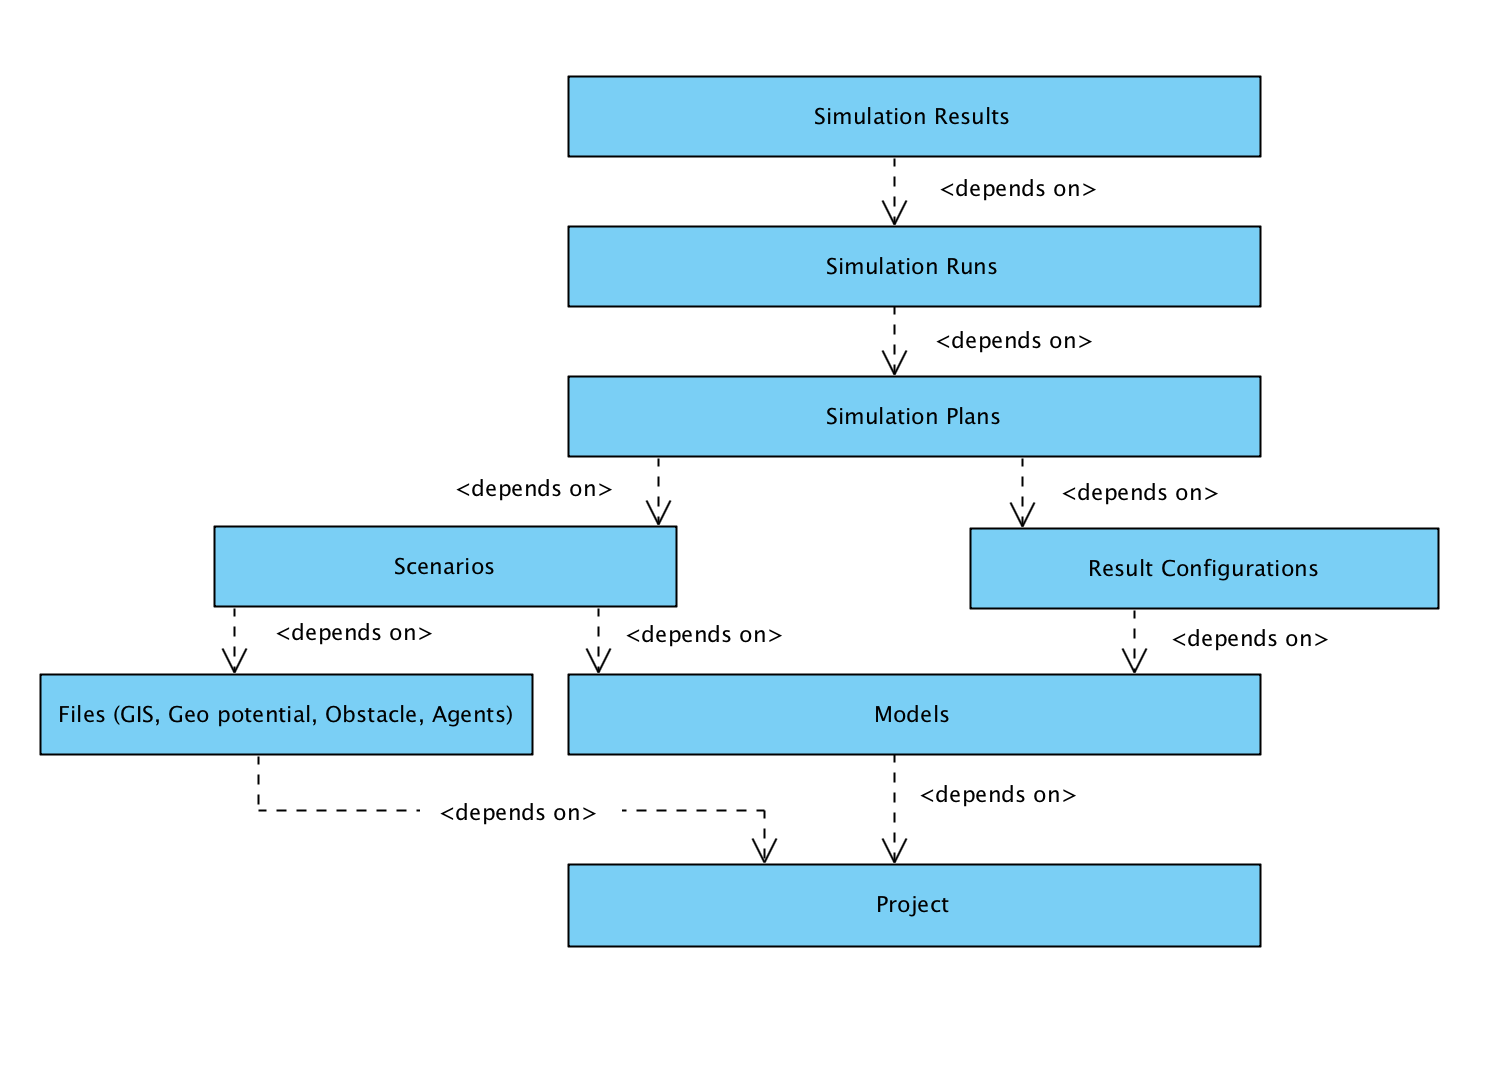
\includegraphics[scale=0.6]{grafiken/marsDependency.png}
            \caption{MARS Resource UML dependency graph}
            \label{fig:marsDependency}
        \end{figure}
        
        Figure \ref{fig:marsDependency} shows the dependencies between MARS resources. It can be observed
        that the order of existence of the resources has to be from the \textbf{project} to the \textbf{simulation} results 
        (bottom to top) when adding a new simulation. Failure to follow this hierarchy results in an
        unsuccessful simulation.

        \begin{figure}[H]
            \centering 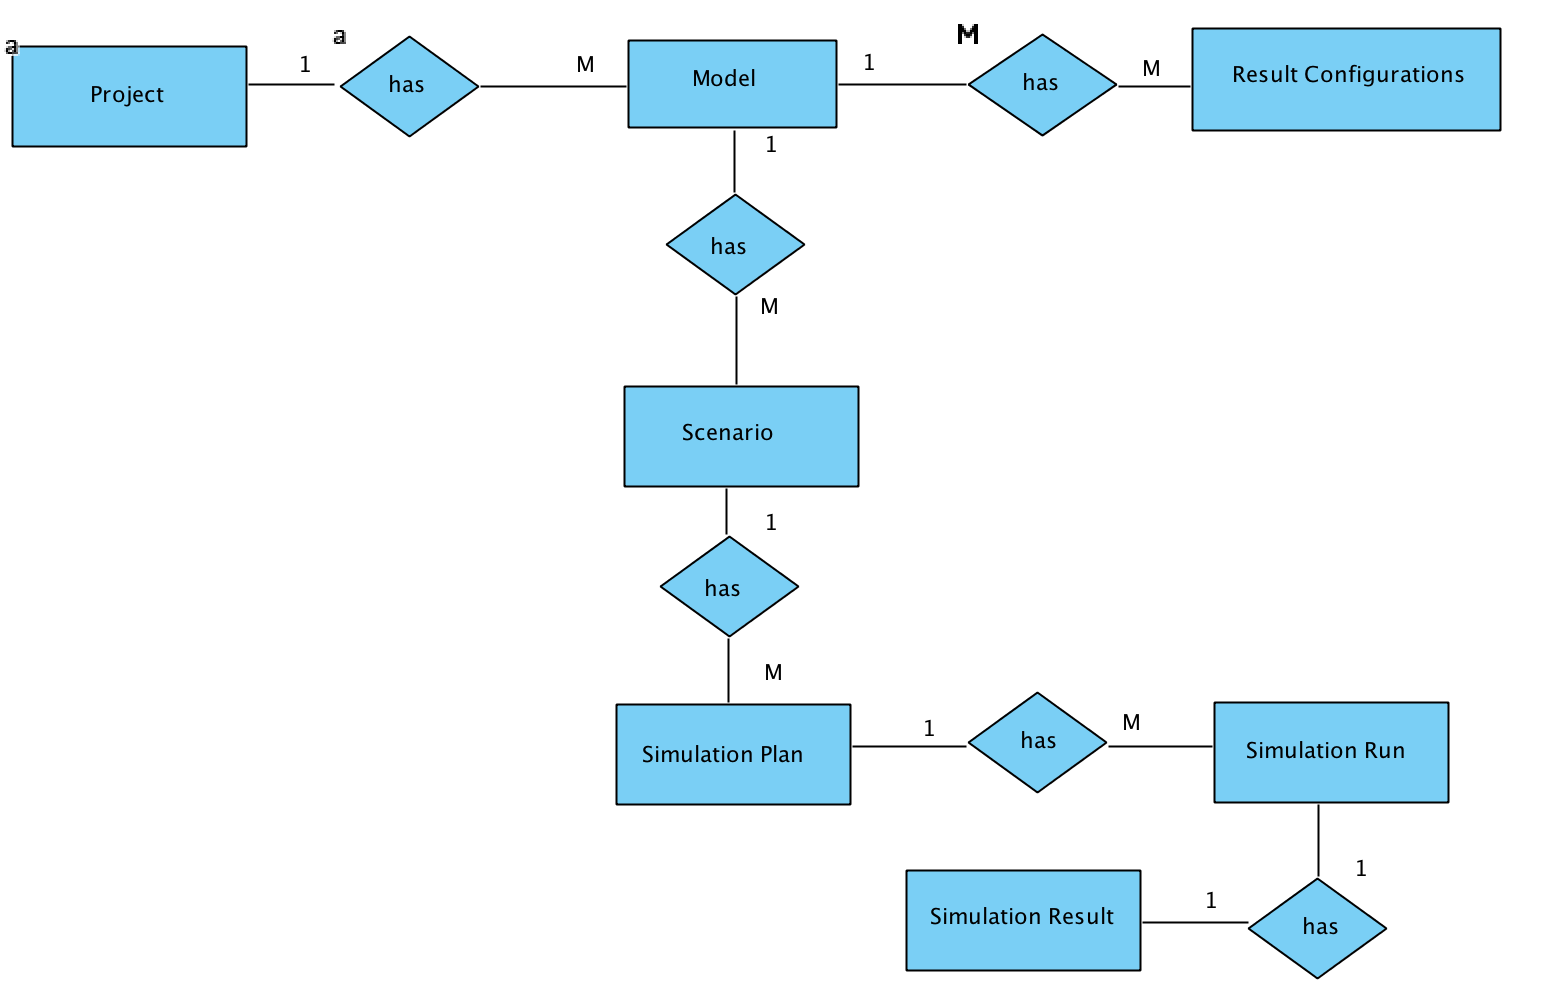
\includegraphics[scale=0.6]{grafiken/ERMars.png}
            \caption{Chen notation Entity Relation Diagram for MARS resources}
            \label{fig:ERMars}
        \end{figure}
        
        Figure \ref{fig:ERMars} shows the data flow of the MARS Resources. From this figure, it is obvious 
        how the resources are dependent upon each other. This follows the hierarchical structure seen in Figure \ref{fig:marsDependency},
        where the project data is at the top, and no other entity can exist without it. A pattern for the cardinality of the entities can be observed.
        The lower level entity can only have a reference to one parent entity, whereas the parent can have multiple children. An exception to this
        pattern is between simulation run and simulation results. A simulation run does not have multiple results because it represents a job which produces
        the output, i.e., simulation results. It is also to be mentioned that every entity except the project is identified as a weak entity because they do not cease
        to exist without its parent entity. 

        \newpage
        Furthermore, the different data flows mentioned in Figure \ref{fig:ERMars} are handled by various services in the MARS framework. 
        Table \ref{table:MARS Resource Hierarchy Service Overview} gives an overview of the elementary services which are responsible for 
        creating and running simulations. For simplicity reasons, only the services
        which have direct dependency with Archive service is mentioned.
        \begin{table}[h!]
            \centering
            \begin{tabular}{|p{4cm}|p{10.5cm}|}
                \hline
                    \textbf{Service Name}  & \textbf{Description}\\
                \hline
                    Project Service & 
                    Handles project resources. \\
                \hline
                    File Service
                    & Handles the import and export of different file resources i.e. models, GIS\footnote{\label{footnote:GIS}GIS: Geographic Information System}, 
                    Time series.\\
                \hline
                    Metadata Service  & Manages all the metadata resources.\\
                \hline
                    Result Config Service  & The Result configurations handles which properties of a model will be stored in the database for a simulation.\\
                \hline
                    Scenario Service  & The Scenario services handles the mapping from the model constructor type to the imported files.\\
                \hline
                    Sim Runner Service  & Handles simulation plans and simulation run.\\
                \hline
                    Database Utility Service  & Handles all the simulation results and is responsible to backup the project data.\\
                \hline
                    Marking Service  & Handles the marking of the resources, so that when the resource is marked by one service it cannot be altered.\\
                \hline
                    Deletion Service  & Handles deletion of the resources.\\
                \hline
            \end{tabular}
            \caption{MARS Resource Hierarchy Elementary Services Overview}
            \label{table:MARS Resource Hierarchy Service Overview}     
        \end{table}    